\documentclass[uplatex,a4paper,dvipdfmx]{jsarticle}
\usepackage{amsfonts, amsmath, amsthm, amssymb}
\usepackage{mathtools}
\usepackage{tikz-cd}
\usepackage{here}
\usepackage{bm}

\renewcommand{\theenumi}{\arabic{enumi}}
\renewcommand{\labelenumi}{(\theenumi) }
\providecommand{\MR}{\relax\ifhmode\unskip\space\fi MR }
%% Theorems
\theoremstyle{plain}
\newtheorem{theorem}{定理}[section]
\newtheorem{conjecture}[theorem]{予想}
\newtheorem{lemma}[theorem]{補題}
\newtheorem{proposition}[theorem]{命題}
\newtheorem{corollary}[theorem]{系}

\theoremstyle{definition}
\newtheorem{definition}[theorem]{定義}
\newtheorem{example}[theorem]{例}
\newtheorem{remark}[theorem]{補足}

%% Some operators
\DeclareMathOperator{\Hom}{\mathrm{Hom}}
\DeclareMathOperator{\Tor}{\mathrm{Tor}}
\DeclareMathOperator{\CHom}{\mathcal{H}\!\mathit{om}}
\DeclareMathOperator{\CTor}{\mathcal{T}\!\mathit{or}}
\DeclareMathOperator{\Auteq}{\mathrm{Auteq}}
\DeclareMathOperator{\Cone}{\mathrm{Cone}}
\DeclareMathOperator{\ev}{\mathrm{ev}}
\DeclareMathOperator{\id}{\mathrm{id}}
\DeclareMathOperator{\depth}{\mathrm{depth}}
\DeclareMathOperator{\Pic}{\mathrm{Pic}}
\DeclareMathOperator{\MCG}{\mathrm{MCG}}
\DeclareMathOperator{\PMCG}{\mathrm{PMCG}}
\DeclareMathOperator{\RHom}{\mathrm{RHom}}
\DeclareMathOperator{\Ker}{\mathrm{Ker}}
\DeclareMathOperator{\Image}{\mathrm{Im}}
\DeclareMathOperator{\Aut}{\mathrm{Aut}}
\DeclareMathOperator{\Inn}{\mathrm{Inn}}
\DeclareMathOperator{\Out}{\mathrm{Out}}
\DeclareMathOperator{\Supp}{\mathrm{Supp}}
\DeclareMathOperator{\SL}{\mathrm{SL}}
\DeclareMathOperator{\Spec}{\mathrm{Spec}}
\DeclareMathOperator{\Perf}{\mathrm{Perf}}
\DeclareMathOperator{\NS}{\mathrm{NS}}
\DeclareMathOperator{\Ext}{\mathrm{Ext}}
\DeclareMathOperator{\Hilb}{\mathrm{Hilb}}
\DeclareMathOperator{\res}{\mathrm{res}}
\DeclareMathOperator{\Ch}{\mathrm{Ch}}
\DeclareMathOperator{\coh}{\mathrm{coh}}
\DeclareMathOperator{\Fuk}{Fuk}
\DeclareMathOperator{\Ob}{Ob}


\newcommand{\nc}{\newcommand}

%% Calligraphic letters

\nc{\cF}{{\mathcal{F}}}
\nc{\cG}{{\mathcal{G}}}
\nc{\cH}{{\mathcal{H}}}

\nc{\cO}{{\mathcal{O}}}
\nc{\cU}{{\mathcal{U}}}
\nc{\cW}{{\mathcal{W}}}

%% Blackboard letters
\nc{\bA}{{\mathbb{A}}}
\nc{\bC}{{\mathbb{C}}}
\nc{\bP}{{\mathbb{P}}}
\nc{\bQ}{{\mathbb{Q}}}
\nc{\bR}{{\mathbb{R}}}
\nc{\bZ}{{\mathbb{Z}}}


\title{代数多様体の導来圏の半捻り関手}
\author{荒井 勇人(東大数理)\thanks{hayato@ms.u-tokyo.ac.jp}}

\begin{document}
\maketitle

\begin{abstract}
	代数多様体$X$の連接層の導来圏$D^b(X)$の自己同値を構成する重要な手法のひとつが、SeidelとThomasにより導入された球面対象$E \in D^b(X)$に沿う捻り関手$T_E \in \mathrm{Auteq} D^b(X)$である。これはホモロジー的ミラー対称性のもとでシンプレクティック多様体上のLagrange球面に沿うDehn捻りに対応する。

	本稿では捻り関手の変種として、ミラー対称性のもとで穴あき曲面の半捻りに対応する$D^b(X)$の自己同値(半捻り関手)を構成し、それを用いて楕円曲面$S$の導来圏の自己同値群$\Auteq D^b(S)$の構造を調べる。

	本稿の内容は著者のプレプリント\cite{2023arXiv230212501A}に基づく。
\end{abstract}

\section{導入}
\subsection{代数多様体の導来圏とホモロジー的ミラー対称性}
$X$を代数多様体とする。
$X$の(連接層の)導来圏$D^b(X)$とは、以下のようにして構成される圏である。

まず$X$上の連接層の有界な複体のなすアーベル圏を$\Ch^b(\coh X)$とする。
\begin{equation}
	\Ch^b(\coh X) = \left\{
	  \begin{tikzcd}
		  E^\bullet \arrow[d, "f^\bullet", name=F]\\
		  F^\bullet
	  \end{tikzcd}
	  \quad = \quad
	  \left(
	  \begin{tikzcd}
			  \cdots \arrow[r] &E^{-1} \arrow[r, "d^{-1}"]\arrow[d, "f^{-1}"] &E^0 \arrow[r, "d^{0}"]\arrow[d, "f^{0}"] &E^1 \arrow[d, "f^{1}"] \arrow[r] &\cdots\\
			  \cdots \arrow[r] &F^{-1} \arrow[r, "d^{-1}"] &F^0 \arrow[r, "d^{0}"] &F^1\arrow[r] &\cdots
		  \end{tikzcd}
	  \right)
	\right\}
\end{equation}


複体の間の射$f^\bullet \colon E^\bullet \to F^\bullet$は、複体のコホモロジーに誘導する射$H^n(f^\bullet) \colon H^n(E^\bullet) \to H^n(F^\bullet)$が全ての$n \in \bZ$について同型であるとき擬同型と呼ばれる。
$X$の連接層の導来圏$D^b(X)$とは、$\Ch^b(\coh X)$を擬同型全体で局所化してできる圏のことである。
これは自然に三角圏の構造を持つ。
定義より$D^b(X)$の対象は$\Ch^b(\coh X)$と同じ連接層の有界複体全体だが、射の構造についてわかりやすく表示するのは簡単ではない。

代数多様体の導来圏は1960年代にGrothendieckと弟子のVerdierによって層係数コホモロジーのSerre双対を一般的に記述する目的で導入された。
成り立ちは技術的な目的によるものだったが、現在では代数幾何学の重要な研究対象の1つとなっている。
ここではその重要性について、多様体の不変量としての側面と、ホモロジー的ミラー対称性における中心概念としての側面から説明する。

一般に空間$X$に対しその不変量を考えることは基本的である。
次元やコホモロジー群などが典型であり、代数多様体であればさらに$K$群、標準環などが挙げられるが、これらの多くが導来圏$D^b(X)$から計算できることが知られている。
また$X$上の連接層全体のなすアーベル圏$\coh X$からは$X$の同型類そのものを復元できるが、$D^b(X)$については以下の2つの定理が示すように$X$を復元できる場合とできない場合がある。
\begin{theorem}[\cite{MR607081}]\label{mukai}
	$X$をAbel多様体とし$\hat{X}$をその双対Abel多様体とする(これらは一般には同型でない)。
	このとき三角圏としての同値$D^b(X) \cong D^b(\hat{X})$が存在する。
\end{theorem}
\begin{theorem}[\cite{MR1818984}]
	$X, Y$を非特異射影多様体とし、$X$の標準束$\omega_X$またはその双対束$\omega_X^\vee$が豊富な直線束(ample line bundle)であると仮定する。
	このとき、導来圏$D^b(X)$と$D^b(Y)$が三角圏として同値であれば、$X$と$Y$は同型である。
\end{theorem}
以上のように$D^b(X)$は$X$の幾何学について非常に多くの情報を持っている一方で、その全てを統制しているわけではない。
その意味で$X$の代わりに$D^b(X)$を考えることは双有理幾何学を考えることに似ている。
双有理幾何学と導来圏の間には実際に深いつながりがあることがわかってきているが、ここでは省略する。


次にミラー対称性とは、ある空間$X$の代数幾何学と別の空間$Y$のシンプレクティック幾何学の間に物理学の超弦理論に由来する不思議な関係があるという現象である。
この結び付きは例えば$X$内の有理曲線の数え上げ問題を$Y$の周期積分に帰着して解決するなど、それまでの代数幾何学にはない、物理学のアイデアに基づく新たな進展をもたらしてきた。
その背後にあるとされる最も強力な予想の1つが、Kontsevichの提唱したホモロジー的ミラー対称性である。
\begin{conjecture}
	Calabi--Yau多様体$X$に対し別のCalabi--Yau多様体$Y$が存在して、$X$の連接層の導来圏$D^b (X)$と$Y$の深谷圏の導来圏$D^b \Fuk(Y)$が(強化)三角圏として同値になる。
\end{conjecture}
ここで深谷圏$\Fuk(Y)$とその導来圏$D^b \Fuk(Y)$はシンプレクティック多様体$Y$に対し定義されるもので、$D^b \Fuk(Y)$の対象と射は大雑把にいうと$Y$のLagrange部分多様体とその交差によって与えられる。
例えば$X$が楕円曲線$E$の場合、そのミラー$Y$はトーラス$T$であり、$E$およびその閉点$x \in E$の構造層$\cO_E, \cO_x \in D^b(E)$がそれぞれ$T$上の緯線と経線に対応する($T$上の曲線はLagrange部分多様体である)。
このようにミラー対称性はまったく異なる種類の幾何学が等価であることを主張する非常に深い現象・予想であり、その背後には導来圏が現れる。
\begin{example}
	楕円曲線とトーラスのミラー対称性において、$\cO_E, \cO_x \in D^b(E)$は$T$上の曲線$\alpha, \beta \in D^b \Fuk(T)$に対応する。$\sum_i \dim \Hom_{D^b(E)}(\cO_E, \cO_x)=1$と$\# (\alpha \cap \beta) = 1$が一致していることは射の対応の帰結である。
	\begin{displaymath}
		\begin{tikzpicture}[samples=300]
			% elliptic curve E
			\draw(-1, 2.5) node{$E$};
			\draw[thick,domain=-1.3247:2] plot(\x,{sqrt(\x^3-\x+1)});
			\draw[thick,domain=-1.3247:2] plot(\x,{-sqrt(\x^3-\x+1)});

			% point on E
			\filldraw[black] (0, 1) circle (3pt);
			\draw(0, 1.3) node[above]{$x$};

			% torus
			\draw(13, 2.5) node{$T$};
			% big square
			\draw[dashed] (5,-2)--(13,-2);
			\draw(9, -2) node{$>$};
			\draw[dashed] (5,2)--(13,2);
			\draw(9, 2) node{$>$};


			\draw[dashed] (5,-2)--(5,2);
			\draw(5, 0) node{\rotatebox{90}{$>>$}};
			\draw[dashed] (13,-2)--(13,2);
			\draw(13, 0) node{\rotatebox{90}{$>>$}};

			% \draw(22, 8) node{$T$};
			% \draw[dashed] (5,0)--(7,0);
			% \draw(14.75, 0) node{$>$};
			% \draw[dashed] (5,0)--(5,8);
			% \draw(5, 6) node{\rotatebox{90}{$>>$}};
			% \draw[dashed] (5,8)--(20,8);
			% \draw(14.75, 8) node{$>$};
			% \draw[dashed] (20,0)--(20,8);
			% \draw(20, 6) node{\rotatebox{90}{$>>$}};

			% horizontal lines
			\draw[ultra thick] (5, -1)--(13, -1);
			\draw(13, -1) node[right]{$\alpha$};
			% \draw[thick] (3, 2)--(5, 2);
			% \draw[thick] (9, 2)--(11, 2);

			% \draw[thick] (0, 0.5)--(11, 0.5);

			% vertical lines
			\draw[ultra thick] (7, -2)--(7, 2);
			\draw(7, 2) node[above]{$\beta$};
		\end{tikzpicture}
		\begin{tikzpicture}[scale=0.5]

		\end{tikzpicture}
	\end{displaymath}
\end{example}
\subsection{導来圏の自己同値群}
導来圏$D^b(X)$の自己同値群$\Auteq D^b(X)$を、三角圏の構造を保つような$D^b(X)$の自己同値関手の同型類がなす群とする。
典型的な自己同値として、$X$の自己同型$f$による逆像$f^*$、$X$上の直線束$L$によるテンソル積$(-)\otimes L$、および三角圏のシフト関手$(-)[1]$が常に存在し、これらの生成する$\Auteq D^b(X)$の部分群
\begin{equation}
	A(X) \coloneq \Aut(X) \ltimes \Pic(X) \times \bZ[1]
\end{equation}
の元は標準的な自己同値と呼ばれる。
自己同値群についてのもっとも基本的な結果は次のBondalとOrlovによる定理である。
\begin{theorem}[\cite{MR1818984}]\label{BO}
	$X$を非特異射影多様体とし、$X$の標準束$\omega_X$またはその双対束$\omega_X^\vee$が豊富な直線束であると仮定する。
	このとき$A(X) = \Auteq D^b(X)$である。
\end{theorem}
この結果により、非自明な包含関係$A(X) \subsetneq \Auteq D^b(X)$が生じうる一番単純な状況は$X$が楕円曲線の場合となる。
このときの$\Auteq D^b(X)$は、Orlovによるアーベル多様体についての結果\cite{MR1921811}を適用すると以下のようになる。
\begin{theorem}[\cite{MR1921811}]
	$X$を楕円曲線とすると、以下の完全列が存在する。
	\begin{equation}\label{eq:autoequivalence_of_elliptic_curve}
		1 \to \Aut{X} \ltimes \Pic^{0}(X)\times \bZ[2] \to \Auteq{D^b(X)} \xrightarrow{\theta} \SL(2, \bZ) \to 1
	\end{equation}
	ここで$\theta$は偶数次のコホモロジー群$H^0(X, \bZ) \oplus H^0(X, \bZ) \cong \bZ^2$への作用で与えられる。
\end{theorem}

さらに$A(X)$の$\theta$による像を具体的に計算することで、楕円曲線の場合には実際に$A(X) \subsetneq \Auteq D^b(X)$となっていることがわかる。
$A(X)$に入らない自己同値は後述する捻り関手によって得られる。

以上の結果がある一方で、それらの適用範囲を除くと導来圏の自己同値群の詳細な記述が得られている多様体の例はそれほど多くはない。
1次元の場合は上記の2つの定理によってすべて理解できているが、2次元の場合定理\ref{BO}の適用できない$K3$曲面や楕円曲面などについては部分的にしかわかっておらず、高次元では結果はさらに少ない。

また導来圏の自己同値はミラー対称性を通じて深谷圏の自己同値と結びつく。
この際興味深いのは、ミラー対称性の同値$D^b \Fuk(Y) \cong D^b (X)$によって$Y$のシンプレクティック同相が$X$の代数多様体としての自己同型に対応するとは限らないということである。
これにより$Y$のシンプレクティック写像類群の作用を$X$側にもってきたときに、$X$の幾何の観点から見て非自明なものが現れうる。
その一例が次に述べるSeidel--Thomasによる捻り関手である。
\subsection{Fourier--向井関手と捻り関手}
Fourier--向井関手(積分関手)とは、積分核と呼ばれる$X \times Y$の導来圏の対象$P \in D^b(X \times Y)$から構成される関手$\Phi^P =\Phi^P_{X \to Y}\colon D^b(X) \to D^b(Y)$である。
$X, Y$を非特異射影多様体とし、$p_X \colon X\times Y \to X, p_Y \colon X \times Y \to Y$を射影とする。
このとき、$P \in D^b(X \times Y)$に対し関手
\begin{equation}
	\Phi^P_{X \to Y} \colon D^b(X) \xrightarrow{p_X^*} D^b(X \times Y) \xrightarrow{ - \otimes P} D^b(X \times Y) \xrightarrow{p_{Y*}} D^b(Y)
\end{equation}
を$P$を積分核とするFourier--向井関手と呼ぶ。
ここで$p_X^*, p_{Y*}, - \otimes P$はそれぞれ逆像、順像、テンソル積(の導来関手)を意味する。

以下の定理より、Fourier--向井関手は導来圏の間の関手、特に同値を調べる上で基本的な道具となる。
\begin{theorem}[\cite{MR1465519}]
	$X, Y$を非特異射影多様体とし、$\Phi \colon D^b(X) \to D^b(Y)$を充満忠実な$\bC$線形三角関手とする。
	このとき$\Phi$はある積分核$P$によるFourier--向井関手$\Phi^P$と同型である。
\end{theorem}
\begin{remark}
	Fourier--向井関手という名前は
	\begin{enumerate}
		\item 対象の対応$\Phi^P(F) = p_{Y*}(p_X^*F \otimes P)$がFourier変換$\cF(f)(\xi) = \int_\bR f(x)\exp(-ix\xi)dx$と似た形をしていること、
		\item 向井\cite{MR607081}によって導入され、導来同値だが同型でない多様体の初めての例の構成(定理\ref{mukai})に使用されたこと
	\end{enumerate}
	に由来する。
\end{remark}
さらにSeidelとThomasは\cite{MR1831820}において、導来圏の自己同値の構成法である捻り関手の概念を導入した。
\begin{theorem}[\cite{MR1831820}]
	$X$を非特異射影多様体とする。
	また$E \in D^b(X)$を球面対象、すなわち\begin{equation}
		E \otimes \omega_X \cong E,\quad \Hom^i(E, E) = \begin{cases}
			\bC & i = 0, \dim X,    \\
			0   & \text{otherwise.}
		\end{cases}
	\end{equation}を満たすものとする。
	このとき$P = \Cone(E^\vee \boxtimes E \xrightarrow{\ev} \cO_\Delta) \in D^b(X \times X)$を積分核とするFourier--向井関手$\Phi^P$は圏同値である。
	これを球面対象$E$に付随する(球面)捻り関手といい、$T_E$と書く。
\end{theorem}
\begin{corollary}
	$E \in D^b(X)$を球面対象とすると、任意の$F \in D^b(X)$について完全三角形
	\begin{equation}\label{eq:twist}
		\Hom^*(E, F) \otimes E \xrightarrow{\ev} F \to T_E F \xrightarrow{+1}
	\end{equation}
	が存在する。
\end{corollary}
この定義のモチベーションについて少し説明する。
Seidelによる一般化Dehn捻り\cite{MR1743463}は、シンプレクティック多様体$M$の中のLagrange球面$S^n$に付随して定義されていた。
捻り関手を一言で表すと、一般化Dehn捻りのミラー対称性のもとでの対応物である。
もう少し詳しく述べると、
Lagrange球面$S^n \subset M$の(導来深谷圏$D^b\Fuk M$の対象としての)自己準同型環は
\begin{align}
	\Hom_{D^b\Fuk M}^*(S^n, S^n) & = HF^*(S^n, S^n)\otimes_\bR \bC
\end{align}
となり、Floerコホモロジー$HF^*(S^n, S^n)$は球面のコホモロジー$H^*(S^n, \bR)$と同型である。
よって、球面対象の2つ目の条件$$\Hom^i(E, E) = \begin{cases}
		\bC & i = 0, \dim X,    \\
		0   & \text{otherwise.}
	\end{cases}$$は$E$の自己準同型環がLagrange球面$S^n$のそれと等しいことを意味する。
さらにSeidelによる同時期の仕事\cite{MR1978046}によって、\eqref{eq:twist}と同様の完全三角形が導来深谷圏へのDehn捻りにおいても成り立つことが示されている。
そこでこれらの球面とDehn捻りの性質をもとに代数的に定義されたのが捻り関手である。
\begin{example}
	\begin{enumerate}
		\item $E$を楕円曲線とすると、$\cO_E$は$D^b(E)$の球面対象である。これによる捻り関手$T_{\cO_E}$は標準的な自己同値ではない自己同値の例を与える。これは楕円曲線とトーラスのミラー対称性のもとで、$\cO_E$に対応するトーラスの緯線に沿ったDehn捻りに対応する。
		\item $S$を代数曲面とし、$\bP^1 \cong C \subset S$を$(-2)$-曲線とする。このとき$C$上の次数$a \in \bZ$の直線束$\cO_C(a)$を$S$上の層とみたものは、(Riemann--Rochの定理より)$D^b(S)$の球面対象である。
	\end{enumerate}
\end{example}
\section{小平ファイバーのミラー対称性と写像類群}
楕円曲面$\pi \colon S \to C$の特異ファイバーとして現れうる曲線は小平とNeronによりADE型のアファインDynkin図形を用いて分類されている。
これらの曲線を小平ファイバーと呼ぶ。
例えば$\rm{I}_n$型と呼ばれる曲線は$n$本の$\bP^1$が$n$角形のかたちに交わってできる特異曲線であり、アファイン$A_n$型Dynkin図形に対応する。



$Y_n$を$\rm{I}_n$型($n \geq 2$)の小平ファイバーとすると、そのミラー多様体は$n$点穴あきトーラス$T_n$であることが\cite{MR3663596}により示されている。
すなわち以下が成り立つ。
\begin{theorem}[\cite{MR3663596}]
	$\cW(T_n)$を$T_n$の巻深谷圏とすると、$\bC$線形三角圏の同値$D^b(Y_n) \cong D^b(\cW(T_n))$が存在する。
\end{theorem}

本稿では深谷圏や巻深谷圏についての詳しい議論は行わないが、この同値によりおおざっぱにいうと$Y_n$上の層とその間の$\Hom$空間の次元が、$T_n$上の曲線とその交差数に対応する。
より正確には、以下が成り立つ。
\begin{theorem}[\cite{2020arXiv201108288O}]
	\begin{enumerate}
		\item シフト関手$[1]$とホモトピーによる違いを除いて、以下のものが1対1対応する。\begin{itemize}
			      \item $D^b(Y_n)$の直既約対象$F$の同型類
			      \item $T_n$上の曲線$\gamma$とその上の直既約$\bC$局所系$V$の組
		      \end{itemize}
		\item (1)の対応で$E,F$と$(\gamma_E, V_E), (\gamma_E, V_F)$が対応し、$E$または$F$がperfectで$\dim V_E = \dim V_F = 1$を満たすとする。このとき\begin{equation}
			      \sum_{i}\dim\Ext^i(E, F) = \#(\gamma_E \cap \gamma_F)
		      \end{equation}が成り立つ。
	\end{enumerate}
\end{theorem}
以下直既約対象$F \in D^b(Y_n)$に対応する曲線を$\gamma_F$で表す。
対象の対応には例えば以下のようなものがある。
\begin{example}\label{correspondence_of_objects}
	$n=3$とする。$Y_3$の既約成分を$G_1, G_2, G_3$とし、それらの上にある非特異閉点を$x_1, x_2, x_3$とする。
	このとき直既約対象$\cO_{Y_3}, \cO_{G_1}, \cO_{G_1}(-1), \cO_{x_1}$などに対応する$T_3$上の曲線は以下の図のような曲線である。
	ただし白い丸は$T_3$の$3$つの穴を表す。
	\begin{displaymath}
		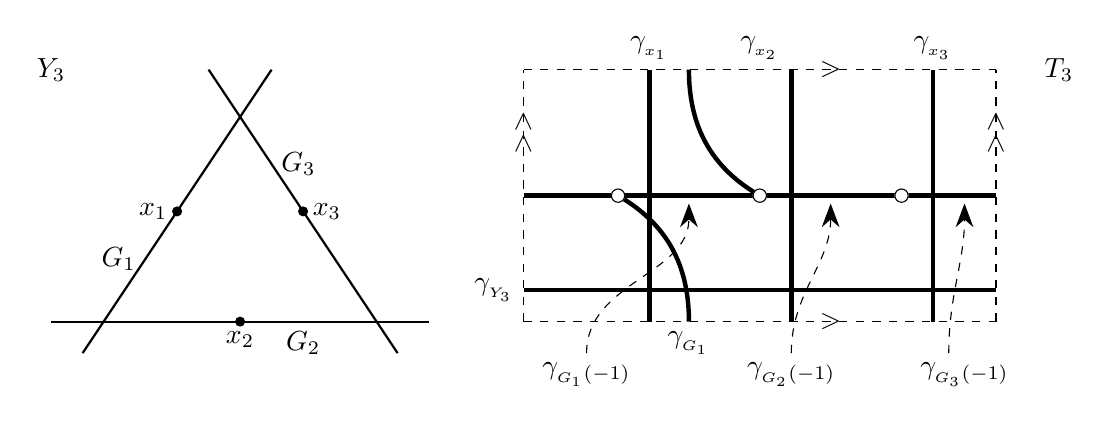
\begin{tikzpicture}[scale = 0.4]
			% fiber
			\draw(-10, 8) node{$Y_3$};
			\draw[thick] (-9,-1)--(-3,8);
			\draw[thick] (-10,0)--(2,0);
			\draw[thick] (1,-1)--(-5,8);

			% points
			\filldraw[black] (-6, 3.5) circle (4pt);
			\filldraw[black] (-4, 0) circle (4pt);
			\filldraw[black] (-2, 3.5) circle (4pt);

			\draw(-6, 3.5) node[left]{$x_1$};
			\draw(-4, 0) node[below]{$x_2$};
			\draw(-2, 3.5) node[right]{$x_3$};

			% components
			\draw(-7, 2) node[left]{$G_1$};
			\draw(-2, 0) node[below]{$G_2$};
			\draw(-3, 5) node[right]{$G_3$};

			% big square
			\draw(22, 8) node{$T_3$};
			\draw[dashed] (5,0)--(20,0);
			\draw(14.75, 0) node{$>$};
			\draw[dashed] (5,0)--(5,8);
			\draw(5, 6) node{\rotatebox{90}{$>>$}};
			\draw[dashed] (5,8)--(20,8);
			\draw(14.75, 8) node{$>$};
			\draw[dashed] (20,0)--(20,8);
			\draw(20, 6) node{\rotatebox{90}{$>>$}};

			% horizontal lines
			\draw[ultra thick] (5, 1)--(20, 1);
			\draw[ultra thick] (5, 4)--(20, 4);
			\draw(5, 1) node[left]{$\gamma_{\cO_{Y_3}}$};
			% \draw[thick] (3, 2)--(5, 2);
			% \draw[thick] (9, 2)--(11, 2);

			% \draw[thick] (0, 0.5)--(11, 0.5);

			% vertical lines
			\draw[ultra thick] (8+1, 0)--(8+1, 8);
			\draw(8+1, 8) node[above]{$\gamma_{\cO_{x_1}}$};
			\draw[ultra thick] (12.5+1, 0)--(12.5+1, 8);
			\draw(12.5, 8) node[above]{$\gamma_{\cO_{x_2}}$};
			\draw[ultra thick] (17+1, 0)--(17+1, 8);
			\draw(17+1, 8) node[above]{$\gamma_{\cO_{x_3}}$};

			% curves
			\draw[ultra thick] (8, 4) to[out=-30,in=90] (10.25, 0);
			\draw[ultra thick] (10.25, 8) to[out=-90,in=150] (12.5, 4);
			\draw(10.25, 0) node[below]{$\gamma_{\cO_{G_1}}$};
			% punctures
			\foreach \u in {8, 12.5, 17}
				{
					\filldraw[white] (\u, 4) circle (6pt);
					\draw[black] (\u, 4) circle (6pt);
				}

			% O_G(-1)
			\draw[dashed, -{Stealth[length=3mm]}] (7, -1) to[out=90, in=-90] (10.25, 3.75);
			\draw(7, -1) node[below]{$\gamma_{\cO_{G_1}(-1)}$};
			\draw[dashed, -{Stealth[length=3mm]}] (13.5, -1) to[out=90, in=-90] (14.75, 3.75);
			\draw(13.5, -1) node[below]{$\gamma_{\cO_{G_2}(-1)}$};
			\draw[dashed, -{Stealth[length=3mm]}] (18.5, -1) to[out=90, in=-90] (19, 3.75);
			\draw(19, -1) node[below]{$\gamma_{\cO_{G_3}(-1)}$};

			% % notations
			% \draw(0, 0.5) node[left]{$\gamma_{\cO_Y}$};
			% \draw(2, 4) node[above]{$\gamma_{\cO_{x_1}}$};
			% \draw(4, 4) node[above]{$\gamma_{\cO_{x_2}}$};
			% \draw(10, 4) node[above]{$\gamma_{\cO_{x_n}}$};

			% \draw(2, 3) node[above left]{$\gamma_{\cO_{G_1}(-1)}$};
			% \draw(1, 3) to[out=-90,in=135](1.5, 2);
			% \draw(4, 3) node[above left]{$\gamma_{\cO_{G_2}(-1)}$};
			% \draw(3, 3) to[out=-90,in=135](3.5, 2);

			% \draw(11, 2) node[right]{$\gamma_{\cO_{G_n}(-1)}$};

		\end{tikzpicture}
	\end{displaymath}
\end{example}
さらにこの対応を用いると、$D^b(Y_n)$の自己同値群について
(楕円曲線の場合と似た)以下の記述が得られる。
\begin{theorem}[{\cite[Theorem D]{2020arXiv201108288O}}]\label{auteq_of_kodaira_fiber}
	完全列
	\begin{equation}
		1 \to \Aut^0(Y_n) \times \Pic^0(Y_n)\times \bZ[1] \to \Auteq{D^b(Y_n)} \xrightarrow{\Upsilon} \MCG(T_n) \to 1
	\end{equation}
	が存在する。
	ただし$\Aut^0$は既約成分を動かさない自己同型、$\Pic^0$は各既約成分上での次数が$0$である直線束の全体を意味する。

	また$\Upsilon$はミラー対称性による対応と以下の意味で整合的である。
	\begin{itemize}
		\item $\Phi \in \Auteq{D^b(Y_n)}$と直既約な$F \in D^b(Y_n)$について、$\Upsilon(\Phi)$は「$F$に対応する曲線」を「$\Phi(F)$に対応する曲線」に写す。
	\end{itemize}
\end{theorem}

さらに$\Upsilon$によって、球面対象$F$に付随する捻り関手$T_F$が曲線$\gamma_F$に付随するDehn捻りに写されることもわかる。
一方で、$\MCG(T_n)$はDehn捻りに加えて穴を結ぶ曲線に沿った半捻りを考えることで生成されることが知られている。
ここで半捻りとは下図のような操作である。

\begin{figure}[h]\label{fig:half_twist}
	\begin{displaymath}
		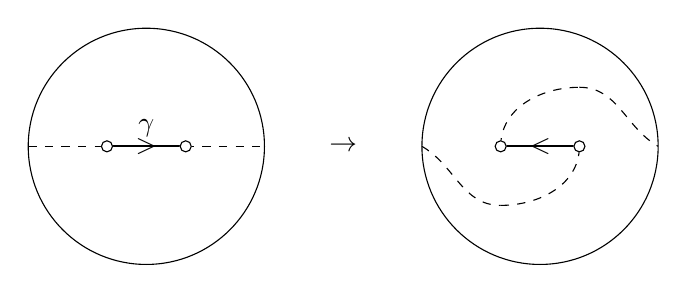
\begin{tikzpicture}
			\draw (0, 1.5) circle[radius=1.5];
			\draw[thick] (-0.5, 1.5)--(0.5, 1.5);
			\draw(0, 1.5) node{$>$};
			\draw[dashed] (-1.5, 1.5)--(-0.5, 1.5);
			\draw[dashed] (0.5, 1.5)--(1.5, 1.5);

			\foreach \u in {-0.5, 0.5}
				{
					\filldraw[white] (\u, 1.5) circle (2pt);
					\draw[black] (\u, 1.5) circle (2pt);
				}
			\draw(0, 1.5) node[above]{$\gamma$};

			\draw(2.5, 1.5) node{$\rightarrow$};

			\draw (0+5, 1.5) circle[radius=1.5];
			\draw[thick] (-0.5+5, 1.5)--(0.5+5, 1.5);
			\draw(5, 1.5) node{$<$};


			\draw[dashed](-1.5+5, 1.5) to[out=-30,in=180](-0.5+5, 0.75);
			\draw[dashed](-0.5+5, 0.75) to[out=0,in=-90](0.5+5, 1.5);

			\draw[dashed](-0.5+5, 1.5) to[out=90,in=180](0.5+5, 2.25);
			\draw[dashed](0.5+5, 2.25) to[out=0,in=150](1.5+5, 1.5);


			\foreach \u in {-0.5, 0.5}
				{
					\filldraw[white] (\u+5, 1.5) circle (2pt);
					\draw[black] (\u+5, 1.5) circle (2pt);
				}
		\end{tikzpicture}
	\end{displaymath}
	\caption{曲線$\gamma$に沿った半捻り}
\end{figure}
そこで半捻りに対応するような導来圏の関手を代数的に定義できるか問うのは自然な疑問である。
本稿の主結果はその構成を与える。
\section{主結果}
% 上述のように、捻り関手はミラー対称性のもとでDehn捻りの対応物を与える。
% では半捻りの対応物がなにかを問うのは自然な疑問である。

本稿の主結果を述べる。1つ目は捻り関手の制限についてのものである。
\begin{theorem}
	$\pi \colon X \to T$を非特異凖射影多様体の間の平坦射とし、$i \colon Y = \pi^{-1}(0) \to X$をファイバーとする。
	また$E \in D^b(Y)$を、$i_*E \in D^b(X)$が球面対象になるような対象とする。
	このとき以下の図式を(自然同型の違いを除いて)可換にするような同値$H_E \colon D^b(Y) \to D^b(Y)$が一意に存在する。
	\begin{equation}
		\begin{tikzcd}
			D^b(Y) \arrow[r,"i_*"]\arrow[d, "H_E"'] & D^b(X) \arrow[d,"T_{i_*E}"]\\
			D^b(Y) \arrow[r, "i_*"]& D^b(X).
		\end{tikzcd}
	\end{equation}
\end{theorem}
\begin{proof}
	積分核$P \in D^b(X \times X)$が$D^b(X \times_T X)$の対象の順像となっているようなFourier--向井関手$\Phi^P$を、相対Fourier--向井関手という。
	その一般論によって、相対Fourier--向井関手はファイバーの導来圏の間の関手に制限できることが知られている。

	よって捻り関手$T_{i_*E}$の積分核$P = \Cone((i_*E)^\vee \boxtimes i_*E \xrightarrow{\ev} \cO_{\Delta_X})$が$D^b(X \times_T X)$の対象の順像になっていることを示せばよく、そのような$D^b(X \times_T X)$の対象は\cite{MR2200048}の議論を参考にすることで具体的に構成できる。
\end{proof}
この定理は、ファイバーからくるような球面対象による捻り関手が、自然にファイバーに「制限」できるということを意味している。
そしてこれを楕円曲面$S$の可約ファイバーの既約成分として現れる$(-2)$-曲線に適用することで、半捻りの類似であるような関手が得られる。
\begin{theorem}
	$\pi \colon S \to C$を楕円曲面とし、$Y_n \subset S$を$\rm{I}_n$型小平ファイバーとする。
	$G \subset Y_n$が$Y_n$の既約成分で$a \in \bZ$のとき、関手$H_{\cO_G(a)} \in \Auteq D^b(Y_n)$は定理\ref{auteq_of_kodaira_fiber}の$\Upsilon \colon \Auteq D^b(Y_n) \to \MCG(T_n)$によって$\gamma_{\cO_G(a)}$に沿った半捻りに写像される。
\end{theorem}
\begin{proof}
	$\Phi = H_{\cO_G(a)}$とおく。
	Dehn--Nielsen--Baerの定理によって、$\MCG(T_n)$の元は$\pi_1(T_n)$への自然な作用により決定される。
	さらに$\pi_1(T_n)$は曲線$\gamma_{\cO_{Y_n}}, \gamma_{\cO_{x_1}}, \dots, \gamma_{\cO_{x_n}}$によって生成される(例\ref{correspondence_of_objects}の図を参照)から、$\Upsilon(\Phi)$がこれらの曲線をどう動かすかを観察すればよい。

	$\Upsilon$の満たすミラー対称性との整合性より、これらの曲線の像はそれぞれ直既約対象$\Phi(\cO), \Phi(\cO_{x_1}), \dots, \Phi(\cO_{x_n}) \in D^b(Y_n)$に対応する曲線となる。
	さらにミラー対称性により、これらの曲線と他の曲線との交点数は導来圏$D^b(Y_n)$での$\Hom$空間の次元と等しいため、ホモロジー代数の基本的な方法で計算できる。
	これにより十分多くの交点数の情報を集めることで、これらの曲線を特定することができ、実際に半捻りと同じ作用を受けていることがわかる。
\end{proof}
\section{楕円曲面の自己同値群}
以上の「半捻り関手」を利用して、あるクラスの楕円曲面の自己同値群の記述を与えることができる。
まず上原\cite{MR3568337}による以下の結果がある。
\begin{theorem}[\cite{MR3568337}]
	\begin{itemize}
		\item $\pi \colon S \to C$を相対的極小な楕円曲面とし、
		\item 小平次元$\kappa(S)$は$0$ではなく、
		\item $\pi$の可約ファイバーはすべて$\rm{I}_n$型($(n \geq 2)$)で、重複ファイバーではないとする。
	\end{itemize}
	さらに部分群$B \subset \Auteq{D^b(S)}$を
	\begin{equation}
		B = \langle T_{\cO_G(a)} \mid G \subset S \text{: $(-2)$-曲線, } a \in \bZ \rangle
	\end{equation}
	と定義する。
	このとき完全列
	\begin{align}
		1 \to \langle B, (-)\otimes \cO_S(D)\mid D.F=0, F \textrm{: ファイバー} \rangle & \rtimes \Aut{S} \times \bZ[2]                      \\
		                                                                                & \to \Auteq{D^b(S)} \xrightarrow{\Theta} \SL(2,\bZ)
	\end{align}
	が存在する。
\end{theorem}
\cite{MR3568337}はさらに$\Theta$の像の特徴づけも与えている。
よってこのような楕円曲面に対しては、$\Auteq D^b(S)$の構造は可約ファイバーの寄与を表す群$B$の構造の研究に帰着されることになる。
これに対し半捻り関手の定義を使うと$B$をファイバーの導来圏の自己同値群と結びつけて考えることができ、ミラー対称性と合わせて以下の結果を得る。
\begin{theorem}
	$\pi \colon S \to C$の可約ファイバー全体を$Y_{n_1}, \dots, Y_{n_l}$とする。
	ここで$Y_{n_j}$は$\rm{I}_{n_j}$型だとする。
	このとき次の完全列が存在する。
	\begin{equation}
		1 \to \langle (-)\otimes \cO_S(Y_{n_j}) \mid j = 1, \dots, l\rangle \to B \to \prod_{j=1}^l \MCG(T_{n_j}).
	\end{equation}
	さらに$B$の像は曲線$\gamma_{\cO_{G_1}(-1)}, \dots, \gamma_{\cO_{G_{n_j}}(-1)}, \gamma_{\cO_{G_1}}, \dots, \gamma_{\cO_{G_{n_j}}} \subset T_{n_j}, 1\leq j \leq l$に付随する半捻りたちによって生成される。
	\begin{figure}[h]
		\centering
		\begin{displaymath}
			\begin{tikzpicture}[scale=1.2]
				% big square
				\draw[dashed] (0,0)--(10,0);
				\draw[dashed] (0,0)--(0,4);
				\draw[dashed] (0,4)--(10,4);
				\draw[dashed] (10,4)--(10,0);

				% horizontal lines
				\draw[thick] (0, 2)--(1, 2);
				\draw[thick] (1, 2)--(3, 2);
				\draw[thick] (3, 2)--(5, 2);
				\draw[thick] (5, 2)--(6, 2);
				\draw[thick] (8, 2)--(9, 2);
				\draw[thick] (9, 2)--(10, 2);


				% vertical lines
				\draw[thick] (0, 4)--(1, 2);
				\draw[thick] (1, 2)--(2, 0);
				\draw[thick] (2, 4)--(4, 0);
				\draw[thick] (4, 4)--(5, 2);
				\draw[thick] (5, 2)--(5.5, 1);
				\draw[thick] (8.5, 3)--(9, 2);
				\draw[thick] (9, 2)--(10, 0);

				% punctures
				\draw[dotted, thick] (5+1.5, 2)--(9-1.5, 2);
				\foreach \u in {1, 3, 5, 9}
					{
						\filldraw[white] (\u, 2) circle (2pt);
						\draw[black] (\u, 2) circle (2pt);
					}

				% notations
				\draw(2, 0) node[below]{$\gamma_{\cO_{G_1}}$};
				\draw(4, 0) node[below]{$\gamma_{\cO_{G_2}}$};
				\draw(10, 0) node[below]{$\gamma_{\cO_{G_{n_j}}}$};

				\draw(2, 3) node[above left]{$\gamma_{\cO_{G_1}(-1)}$};
				\draw(1, 3) to[out=-90,in=135](1.5, 2);
				\draw(4, 3) node[above left]{$\gamma_{\cO_{G_2}(-1)}$};
				\draw(3, 3) to[out=-90,in=135](3.5, 2);

				\draw(10, 2) node[right]{$\gamma_{\cO_{G_{n_j}}(-1)}$};

			\end{tikzpicture}
		\end{displaymath}
		\caption{曲線$\gamma_{\cO_{G_1}(-1)}, \dots, \gamma_{\cO_{G_{n_j}}(-1)}, \gamma_{\cO_{G_1}}, \dots, \gamma_{\cO_{G_{n_j}}} \subset T_{n_j}$}
	\end{figure}
\end{theorem}
\bibliographystyle{amsalpha}
\bibliography{half_twist}
\end{document}